\chapter{Foundation Of Distributed Data Systems}
\label{chapter_technical_foundation}
\setlength{\epigraphwidth}{0.95\textwidth}
\setlength\epigraphrule{0pt}
\epigraph{\itshape ``I'm not telling you it's going to be easy - I'm telling you it's going to be worth it.''}{--- Arthur L. Williams Jr., \textit{Founder of Primerica Financial Services}}

In this chapter we will go trough the foundation of data systems, requirements and concepts which apply to any (data-driven) system. This covers in particular following topics:
\begin{samepage}
\begin{itemize}
	\item Section\ref{tf_nfreq} Requirements of \textbf{\nameref{tf_nfreq}}, e.g. 
		\begin{itemize}
			\item \ref{tf_nfreq_scalability} \nameref{tf_nfreq_scalability}, 
			\item \ref{tf_nfreq_avrel} \nameref{tf_nfreq_avrel}, 
			\item \ref{tf_nfreq_maintainability} \nameref{tf_nfreq_maintainability}, 
			\item \ref{tf_nfreq_extensability} \nameref{tf_nfreq_extensability} amongst others.
		\end{itemize}
	\item Section \ref{tf_storageconcepts} \textbf{\nameref{tf_storageconcepts}} for databases
	\item Section \ref{tf_dma} \textbf{\nameref{tf_dma}} concepts
	\item Section \ref{tf_dds} \textbf{\nameref{tf_dds}}, e.g.
		\begin{itemize}
			\item \ref{tf_dds_partitioning} \nameref{tf_dds_partitioning}, 
			\item \ref{tf_dds_replication} \nameref{tf_dds_replication}, 
			\item \ref{tf_dds_transactions} \nameref{tf_dds_transactions}, 
			\item \ref{tf_dds_consistency} \nameref{tf_dds_consistency} amongst others.\\
		\end{itemize}
\end{itemize}
\end{samepage}

At the end you will have a basic understanding about the difference between common and distributed systems and databases, the basic concepts of each of them and which one theoretically fits best to solve a certain problem.
A more hands-on deep-dive into related software, frameworks as well as specific problems and use cases will be demonstrated later in chapter XXX.

\section{Data-Driven Systems}
\label{tf_nfreq}
When we think about data-driven systems, we mostly think about the same requirements we expect of any other data system we already know:
\begin{itemize}
	\item \textbf{Data Storage}: We need to store data and also need to be able to find it again later (\textit{database}). 
	\item \textbf{Data Querying}: We need to be able to query and filter data efficiently in certain kinds of ways (\textit{transaction and indices}).
	\item \textbf{Retention and Performance}: We want results fast, especially of expensive read operations (\textit{caching}).
	\item \textbf{Data Processsing}: We want to be able to process a huge amount of data (\textit{batch processing}) as well as process data asynchronously (\textit{stream processing}).\\
\end{itemize}

This sounds quite obvious, but remember those requirements are still the same as for the first database CODASYL\footnote{https://en.wikipedia.org/wiki/CODASYL} back in the 1960's. Even though there are and have been a lot of databases back in time, each of them with a diverse purpose and different approaches to solve e.g. indexing or caching - all of them still match those same requirements. Certainly those data systems evolved much further, especially within the last years, you may noticed:
\begin{itemize}
	\item Relational Databases being able to handle NoSQL data (e.g. even ``retirees'' like IBM DB2\footnote{\cite{IBMDB2JS}, https://www.ibm.com/support/knowledgecenter/en/SSEPEK\_11.0.0/json/src/tpc\\/db2z\_jsonfunctions.html} or Oracle\footnote{\cite{ORCLJS}, https://docs.oracle.com/database/121/ADXDB/json.htm}) as well as NoSQL databases being able to handle traditional SQL (e.g. ToroDB\footnote{\cite{TORODB}, https://www.torodb.com}) or
	\item databases becoming message queues (e.g. RethinkDB\footnote{\cite{RDBMQ}, https://rethinkdb.com/docs/changefeeds/} or Redis\footnote{\cite{RUDMQ}, https://redis.io/commands/rpoplpush}\footnote{\cite{BSARN}, see 5. Adopting Redis for Application Data}) and the other way around message queueing systems become databases (e.g. Apache Kafka\footnote{\cite{KFKQU}, https://kafka.apache.org/10/documentation/streams/developer-guide/interactive-queries.html}).\\
\end{itemize}

As you can see, boundaries between traditional databases and data-driven applications get blurred and in the same way more diversified. 
There is no one-size-fits-all solution, e.g. like you can find back in the past in the 1990's or early 2000s. 
At that time monolithic single-, 2 and 3-tier, architectures were state-of-the-art (see Figure \ref{schema_application_architectures} left-hand side). \\
Usually the \textbf{database layer} was represented by a data store like MySQL, Oracle, DB2 or even just files containing data stored on the local disk.\\
The \textbf{application layer} was usually a monolithic application developed in languages like PHP, Perl, C++ or Java and running on a web- or application server (e.g. Apache HTTP Server or IBM WebSphere).\\
And last but not least the \textbf{client layer}: a web browser like nowadays.\\
\begin{figure}[ht]
	\centering
  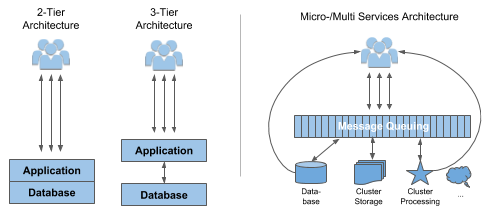
\includegraphics[width=1\textwidth]{application_architectures.png}
	\caption{Schema - Application Architectures}
	\label{schema_application_architectures}
\end{figure}
If you take a look at Figure \ref{schema_ebay_architecture_1997_1999} on page \pageref{schema_ebay_architecture_1997_1999} you can see an example of this time you may know: ebay.com. They have used the classical 3-tier architecture as well: Oracle as the database running on Solaris as OS\footnote{OS, Operating System}\abk{OS}{Operating System}, C++ as application code running on the Microsoft IIS\footnote{\cite{IIS}, \textit{Microsoft Internet Information Services, an extensible web server created by Microsoft for use with the Windows NT family.}} web server.
\begin{figure}[ht]
	\centering
  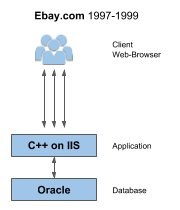
\includegraphics[width=0.4\textwidth]{ebay_architecture_199799.png}
	\caption{Schema - Architecture Ebay.com 1997-1999}
	\label{schema_ebay_architecture_1997_1999}
\end{figure}
As you can already guess, this architecture won't scale very well today, in fact the only way to scale this application was to upgrade the single server (\textit{scale up vertically}), in case of ebay.com they once switched from commodity hardware to a very pricey mainframe server (Sun Enterprise E10000\footnote{\cite{EBAYA}, slide 11}) to buy some time. But as you may have noticed there are much more ovious issues, e.g. if you think about:
\begin{itemize}
	\item \textbf{Redundancy} does not exist at all (if the database itself or it's server suffers an outage the whole system will be unavailable.
	\item \textbf{Extensability} is not existent, the system is only able to scale up vertically and if this is needed, a downtime is inevitable, as no part of the data system is neither replicated nor virtualized.
	\item \textbf{Maintainablity} is also very limited as any maintenance of the database will require a certain amount of time in which the application will be unavailable.
\end{itemize}
But we will dicuss this later in the following chapters.\\

The previously mentioned issues are already sufficient reason but also the increasing amount of data as well as required features of data systems these days (becoming more diversified in the same way) make it unfeasible to rely on a single tool. Instead each functionality is usually broken down into parts which can be done efficiently by suitable tools which are sticked together within the applications itself. This could probably look like as you can see in Figure \ref{schema_application_architectures} (right-hand side) on page \pageref{schema_application_architectures}, but that's just one plain example of many other.\\

Instead of having one single-purpose data store, there are several tied together, each one of them to fulfill it's specific part within the whole data system but all of them tied together as one application. \\
As you can see one part of the data system could be: a \textbf{database} (like you saw in Figure \ref{schema_ebay_architecture_1997_1999} on page \pageref{schema_ebay_architecture_1997_1999}), e.g. to store and serve:\\
\begin{itemize}
	\item user data (e.g. in case of an application with login)
	\item product data (e.g. in case the applications is a web shop)
	\item user generated content  (e.g. in case the application is a newspage, blog or forum)\\
\end{itemize}
Another part could be \textbf{cluster storage} like Hadoop, which could:\\
\begin{itemize}
	\item keep a complete history of all raw data (e.g. page requests of a website or measured values of a sensor)
	\item serve for batch processing (e.g. crunching the whole history of data, which is impossible for a single database, as it couldn't even save the whole data and certainly wouldn't be able to process it later on)
	\item serve for analytic and reporting purposes (e.g. reports of how many people have visited the website within the last year based on the raw data)\\
\end{itemize}
Also frequently seen, an analytical \textbf{cluster processing engine}, e.g. Spark or Flink to:\\
\begin{itemize}
	\item process data gathered in real-time (e.g. every page request of a website) for analytical purposes
	\item use processed data, to run data science models on it (e.g. to serve targeted advertisements or customized content to a user on a website, based on his last page requests, browser user-agent or device)
	\item ...\\
\end{itemize}
\begin{figure}[ht]
	\centering
  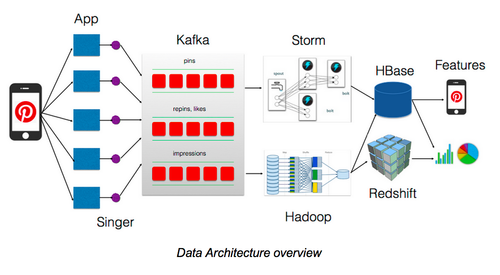
\includegraphics[width=1\textwidth]{pinterest_architecture.png}
	\caption{Schema - Architecture pinterest.com}
	\label{schema_pinterest_architecture}
\end{figure}
If you take a look at Figure \ref{schema_pinterest_architecture}, you can see a comparable data system architecture, implemented by pinterest.com\footnote{\cite{PINA}, Architecture of Giants: Data Stacks at Facebook, Netflix, Airbnb, and Pinterest}. Redis as a database on top of the hadoop cluster storage to serve for analytical purposes (e.g. ad serving of pinterest's adbuyers) or HBase on top of Hadoop cluster storage and Storm to serve features for the actual end-user of pinterest.com.\\

But we need to take care here: by creating new and more complex data systems from special purpose data systems, complexity is growing with it. How to ensure the system is avalaible with a reliable performance if something crashes? How to make sure data remains consistent and complete if things go wrong? How to scale the data system to be able to handle increased load?...\\
There are many apects which are crucial and influence the architecture of a data system like regulary constraints like data security, location of servers, SLA's\footnote{\cite{WKSLA}, \textit{Service Level Agreement, a commitment between a service provider and a client. Particular aspects of the service – quality, availability, responsibilities – are agreed between the service provider and the service user.}}\abk{SLA}{Service Level Agreement} or existing devlopment and operation skills - which very much depend on the specific situation.\\
Within the next chapters we will focus on the aspects which must be taken into account by any data system:

\begin{itemize}
			\item \nameref{tf_nfreq_scalability} (Chapter \ref{tf_nfreq_scalability}),
			\item \nameref{tf_nfreq_avrel} (Chapter \ref{tf_nfreq_avrel}),
			\item \nameref{tf_nfreq_maintainability} (Chapter \ref{tf_nfreq_maintainability}) and
			\item \nameref{tf_nfreq_extensability} (Chapter \ref{tf_nfreq_extensability}).\\
\end{itemize}

As many people and companies usually mess around with those terms, firstly we will develop a clear understanding on what they mean and later on take a closer look on how to apply algorithms, development and architectures to fulfill them appropriately.

\subsection{Scalability}
\label{tf_nfreq_scalability}
As is evident from the introduction of this chapter: the fact that a system is working reliable today doesn't mean it will necessarily work reliable in the future. The data system of ebay.com in 1999 was maxed out at handling \textbf{50.000} active listings\footnote{\cite{EBAYA}, slide 9}, imagine how the system would behave today at handling \textbf{1 billion} active listings\footnote{\cite{EBAYHP}}.
Obviously handling increased load (e.g. a larger amount of data needed to store or request to handle) is a major factor of a scalable data system.
\\[0.5 cm]
\hspace*{4mm}%
\fbox{%
  \hspace*{1.5mm}\hspace*{-1\fboxsep}%
  \parbox{0.08\textwidth + 5mm - 2\fboxsep}{%
\begin{minipage}{0.1\textwidth}
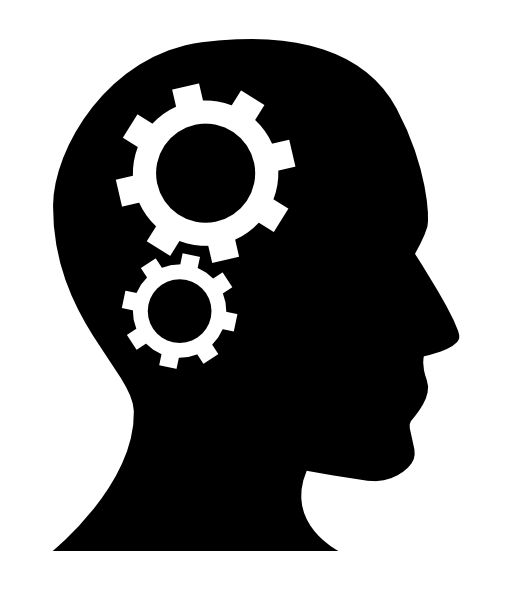
\includegraphics[width=\linewidth]{gear_brain.png}
\end{minipage}
  }%
}\hspace*{4mm}%
\begin{minipage}{0.8\textwidth}\raggedright
\textbf{Scalability} is the capability of data system to handle a growing amount of load (e.g. a larger amount of data needed to store or requests to handle). A data system is considered scalable if its capable of increasing it's total through-/output under an increased load when resources (typically hardware) are added. \\
\end{minipage}\\[0.4 cm]

Note that, ``\textit{scalability}'' isn't a binary tag that could be attached to a data system. It's pointless to say ``\textit{a data system is scalable}'' as well as ``\textit{a data system is not scalable}'', in either way you must think about ``\textit{If the load of a data system grows in a certain way, what are the options on the table for coping with the growth?}'' and ``\textit{How can we add ressources (hardware) to be able to handle the additional load?}''. \\
Therefore we will discuss the parameters and definition of \textbf{Load} (Section \ref{tf_nfreq_scalability_load}) and \textbf{Performance} (Section \ref{tf_nfreq_scalability_performance}) within the next section as well as \textbf{Approaches} for coping with load to achieve a certain performance (Section \ref{tf_nfreq_scalability_approaches}).

\subsubsection{Load}
\label{tf_nfreq_scalability_load}
To get an idea what \textit{load} of a data system actually means, how it could be described an measured, we will take a nother look at the example of ebay.com discussed so far. If we take a look back at the architecure of ebay at 1997-1999 (Figure \ref{schema_ebay_architecture_1997_1999} on page \pageref{schema_ebay_architecture_1997_1999}) we can already guess with increasing load (page requests to certain items listed on ebay.com and in this way calls to the database through the application) will reach its limit at the maximum amount of read requests the oracle database can serve. As the application tier (web server) has already been scaled horizontally to multiple nodes, the oracle database server reached its limit of physical growth in November 1999. So ebay added an additional server to not just elmininate the SPOF\abk{SPOF}{Single Point Of Failure}\footnote{\cite{WPSPOF}, Single Point Of Failure} to be able to failover but also they have splitted the database to be able to logically partition it into separate instances and in this way be able to scale horizontally. This was achieved in 2001 by splitting items by categories, as you can see in Figure XXX. In this simple way it was possible to distribute the load (mostly page requests for items) in an ``equal'' way to different physical nodes.
Later on they segmented whole databases into functional areas like hosts for item, user, account or transaction data as well as partition the data by typical usage characteristics to scale horizontally.\\

They obviously did furher optimizations at the whole data system to be able to cope with the increasing load, like disabling transactions, moving CPU-intensive\abk{CPU}{Central Processing Unit}\footnote{CPU, In computing, a processor or processing unit is an electronic circuit which performs operations on some external data source, usually memory or some other data stream is called central processing unit} work to the application tier (e.g. joins, referential integrity or sorting), extensive use of prepared statements...but as this techniques are not mainly specific for distributed systems and some of them not even recommened nowadays, we won't focuse on them within this lecture.\\

In the example of ebay.com, requests per item and category could be a valuable \textit{load parameter} for discussing scalability, since it determines the database requests per data record and partition - as proven by the the data system structure of ebay at 2002 as we see.
Your or other data systems you have seen so far most likely have very different characteristics, but you can apply similar principles to reason about their load.
\\[0.5 cm]
\hspace*{4mm}%
\fbox{%
  \hspace*{1.5mm}\hspace*{-1\fboxsep}%
  \parbox{0.08\textwidth + 5mm - 2\fboxsep}{%
\begin{minipage}{0.1\textwidth}
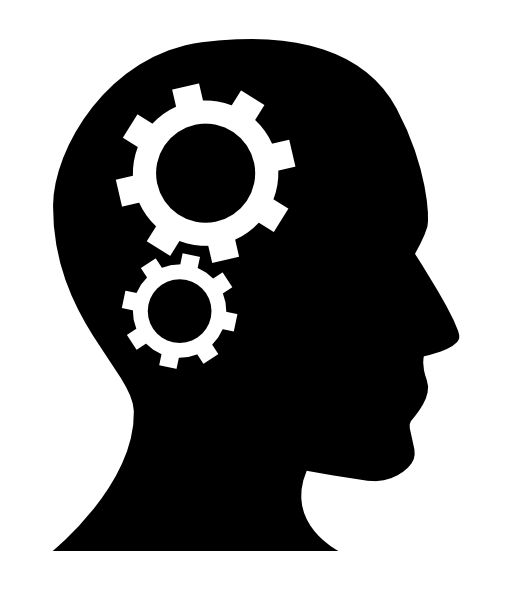
\includegraphics[width=\linewidth]{gear_brain.png}
\end{minipage}
  }%
}\hspace*{4mm}%
\begin{minipage}{0.8\textwidth}\raggedright
The \textbf{load} of a data system is a measurement of the amount of computational work it performs (depending on the architecture in-place), e.g. the number of (concurrent) reads from a data storage, writes to a data storage or the ratio between reads and writes. The maximum load is defined by the weakest part of the architecture (=\textit{bottleneck}). \\[0.4 cm]
\end{minipage}\\

\subsubsection{Performance}
\label{tf_nfreq_scalability_performance}
Now that we have described what \textit{load} of a data system means as well as what \textit{load parameters} could be, we will examine more closely what happens when the load increases. Usually there are two important cases you need to think about while developing data systems:\\
\begin{itemize}
			\item The load parameter increases, but all ressources (e.g. number of server, CPU or memory) stay the same - how is the performance of the data system affected?
			\item The load parameter increases - how much do you need to increase the ressources (e.g. number of server, CPU or memory) to keep the performance stay the same?\\
\end{itemize}

But how to answer them? Therefore we need performance numbers. In case of data systems measurement, methods usually are \textbf{throughput} (number of records that can be handled), e.g.:
\begin{itemize}
			\item read/writes per second (in case of MongoDB up to 100.000 read/writes per second)
			\item messages processed (in case of Apache Kafka and Linkedin more than 2 million records per second on just 3 nodes)
			\item data processed (in case of Apache Hadoop and MapReduce terabytes of data within several seconds)\\
\end{itemize}

or if your buidling a data-system which works as the backend of a end-user facing application like a website, it's more about the \textbf{response time}, which means the time between sending a request and receiving the response. For instance if we think about the example of ebay.com within the previous chapters, as of 2016 they had 1 billion items accessible at any time, needed to serve 2 billion page requests each day and had to fulfill each of them within fractions of a second. \\

Regardless of throughput or response time - if we think about performance we don't think about a single number, but a distribution of values that we can measure. If you will repeat the same page request, read or writes on the same data system: response time and throughput will inevitable vary somehow. There are simply too many factors you usually cannnot contain:
\begin{itemize}
			\item network issues (e.g. latency or TCP packet loss and retransmission)
			\item os issues (e.g. a page faults, context switches or running background processes)
			\item physical issues (e.g. a damaged disk/ssd or overheating of a CPU and, associated therwith a decreased processing power) \\
\end{itemize}


Text
\\[0.5 cm]
\hspace*{4mm}%
\fbox{%
  \hspace*{1.5mm}\hspace*{-1\fboxsep}%
  \parbox{0.08\textwidth + 5mm - 2\fboxsep}{%
\begin{minipage}{0.1\textwidth}
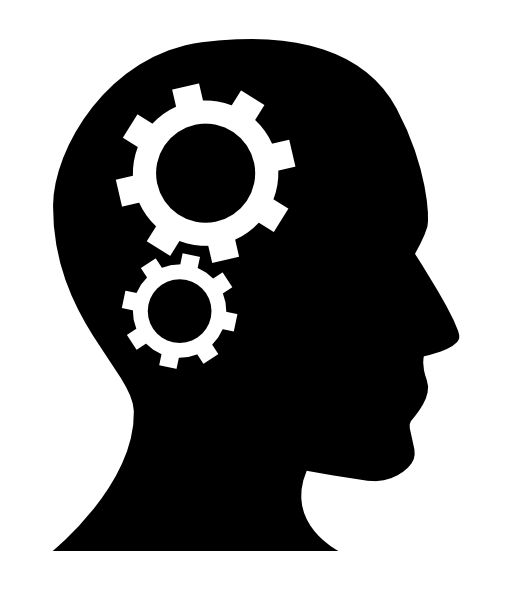
\includegraphics[width=\linewidth]{gear_brain.png}
\end{minipage}
  }%
}\hspace*{4mm}%
\begin{minipage}{0.8\textwidth}\raggedright
\textbf{Performance} of a data system is defined by system throughput and response time, e.g. number of transactions (like read/write operations), processed records (like aggregations for analytical purposes) or even system commands (like an \textit{update statistics} or rebalancing of several data nodes) under a given workload and for a specific timeframe. It usually depends on a variety of influencable as well as uninfluencable factors of the system itself, like network latency, a page fault or damaged disk. \\[0.4 cm]
\end{minipage}\\

\subsubsection{Approaches}
\label{tf_nfreq_scalability_approaches}

\subsection{Availablity/Reliabaility}
\label{tf_nfreq_avrel}
Lorem ipsum dolor sit amet, consetetur sadipscing elitr, sed diam nonumy eirmod tempor invidunt ut labore et dolore magna aliquyam erat, sed diam voluptua. At vero eos et accusam et justo duo dolores et ea rebum. Stet clita kasd gubergren, no sea takimata sanctus est Lorem ipsum dolor sit amet. Lorem ipsum dolor sit amet, consetetur sadipscing elitr, sed diam nonumy eirmod tempor invidunt ut labore et dolore magna aliquyam erat, sed diam voluptua. At vero eos et accusam et justo duo dolores et ea rebum. Stet clita kasd gubergren, no sea takimata sanctus est Lorem ipsum dolor sit amet.

\subsection{Maintainability}
\label{tf_nfreq_maintainability}
Lorem ipsum dolor sit amet, consetetur sadipscing elitr, sed diam nonumy eirmod tempor invidunt ut labore et dolore magna aliquyam erat, sed diam voluptua. At vero eos et accusam et justo duo dolores et ea rebum. Stet clita kasd gubergren, no sea takimata sanctus est Lorem ipsum dolor sit amet. Lorem ipsum dolor sit amet, consetetur sadipscing elitr, sed diam nonumy eirmod tempor invidunt ut labore et dolore magna aliquyam erat, sed diam voluptua. At vero eos et accusam et justo duo dolores et ea rebum. Stet clita kasd gubergren, no sea takimata sanctus est Lorem ipsum dolor sit amet.

\subsection{Extensability}
\label{tf_nfreq_extensability}
Lorem ipsum dolor sit amet, consetetur sadipscing elitr, sed diam nonumy eirmod tempor invidunt ut labore et dolore magna aliquyam erat, sed diam voluptua. At vero eos et accusam et justo duo dolores et ea rebum. Stet clita kasd gubergren, no sea takimata sanctus est Lorem ipsum dolor sit amet. Lorem ipsum dolor sit amet, consetetur sadipscing elitr, sed diam nonumy eirmod tempor invidunt ut labore et dolore magna aliquyam erat, sed diam voluptua. At vero eos et accusam et justo duo dolores et ea rebum. Stet clita kasd gubergren, no sea takimata sanctus est Lorem ipsum dolor sit amet.


\section{Storage Concepts}
\label{tf_storageconcepts}
Lorem ipsum dolor sit amet, consetetur sadipscing elitr, sed diam nonumy eirmod tempor invidunt ut labore et dolore magna aliquyam erat, sed diam voluptua. At vero eos et accusam et justo duo dolores et ea rebum. Stet clita kasd gubergren, no sea takimata sanctus est Lorem ipsum dolor sit amet. Lorem ipsum dolor sit amet, consetetur sadipscing elitr, sed diam nonumy eirmod tempor invidunt ut labore et dolore magna aliquyam erat, sed diam voluptua. At vero eos et accusam et justo duo dolores et ea rebum. Stet clita kasd gubergren, no sea takimata sanctus est Lorem ipsum dolor sit amet.


\section{Data Models And Access}
\label{tf_dma}
Lorem ipsum dolor sit amet, consetetur sadipscing elitr, sed diam nonumy eirmod tempor invidunt ut labore et dolore magna aliquyam erat, sed diam voluptua. At vero eos et accusam et justo duo dolores et ea rebum. Stet clita kasd gubergren, no sea takimata sanctus est Lorem ipsum dolor sit amet. Lorem ipsum dolor sit amet, consetetur sadipscing elitr, sed diam nonumy eirmod tempor invidunt ut labore et dolore magna aliquyam erat, sed diam voluptua. At vero eos et accusam et justo duo dolores et ea rebum. Stet clita kasd gubergren, no sea takimata sanctus est Lorem ipsum dolor sit amet.

\section{Challenges Of Distributed Data Systems}
\label{tf_dds}
Lorem ipsum dolor sit amet, consetetur sadipscing elitr, sed diam nonumy eirmod tempor invidunt ut labore et dolore magna aliquyam erat, sed diam voluptua. At vero eos et accusam et justo duo dolores et ea rebum. Stet clita kasd gubergren, no sea takimata sanctus est Lorem ipsum dolor sit amet. Lorem ipsum dolor sit amet, consetetur sadipscing elitr, sed diam nonumy eirmod tempor invidunt ut labore et dolore magna aliquyam erat, sed diam voluptua. At vero eos et accusam et justo duo dolores et ea rebum. Stet clita kasd gubergren, no sea takimata sanctus est Lorem ipsum dolor sit amet.

	\subsection{Partitioning}
	\label{tf_dds_partitioning}
	Lorem ipsum dolor sit amet, consetetur sadipscing elitr, sed diam nonumy eirmod tempor invidunt ut labore et dolore magna aliquyam erat, sed diam voluptua. At vero eos et accusam et justo duo dolores et ea rebum. Stet clita kasd gubergren, no sea takimata sanctus est Lorem ipsum dolor sit amet. Lorem ipsum dolor sit amet, consetetur sadipscing elitr, sed diam nonumy eirmod tempor invidunt ut labore et dolore magna aliquyam erat, sed diam voluptua. At vero eos et accusam et justo duo dolores et ea rebum. Stet clita kasd gubergren, no sea takimata sanctus est Lorem ipsum dolor sit amet.

	\subsection{Replication}
	\label{tf_dds_replication}
	Lorem ipsum dolor sit amet, consetetur sadipscing elitr, sed diam nonumy eirmod tempor invidunt ut labore et dolore magna aliquyam erat, sed diam voluptua. At vero eos et accusam et justo duo dolores et ea rebum. Stet clita kasd gubergren, no sea takimata sanctus est Lorem ipsum dolor sit amet. Lorem ipsum dolor sit amet, consetetur sadipscing elitr, sed diam nonumy eirmod tempor invidunt ut labore et dolore magna aliquyam erat, sed diam voluptua. At vero eos et accusam et justo duo dolores et ea rebum. Stet clita kasd gubergren, no sea takimata sanctus est Lorem ipsum dolor sit amet.

	\subsection{Transactions}
	\label{tf_dds_transactions}
	Lorem ipsum dolor sit amet, consetetur sadipscing elitr, sed diam nonumy eirmod tempor invidunt ut labore et dolore magna aliquyam erat, sed diam voluptua. At vero eos et accusam et justo duo dolores et ea rebum. Stet clita kasd gubergren, no sea takimata sanctus est Lorem ipsum dolor sit amet. Lorem ipsum dolor sit amet, consetetur sadipscing elitr, sed diam nonumy eirmod tempor invidunt ut labore et dolore magna aliquyam erat, sed diam voluptua. At vero eos et accusam et justo duo dolores et ea rebum. Stet clita kasd gubergren, no sea takimata sanctus est Lorem ipsum dolor sit amet.

	\subsection{Consistency}
	\label{tf_dds_consistency}
	Lorem ipsum dolor sit amet, consetetur sadipscing elitr, sed diam nonumy eirmod tempor invidunt ut labore et dolore magna aliquyam erat, sed diam voluptua. At vero eos et accusam et justo duo dolores et ea rebum. Stet clita kasd gubergren, no sea takimata sanctus est Lorem ipsum dolor sit amet. Lorem ipsum dolor sit amet, consetetur sadipscing elitr, sed diam nonumy eirmod tempor invidunt ut labore et dolore magna aliquyam erat, sed diam voluptua. At vero eos et accusam et justo duo dolores et ea rebum. Stet clita kasd gubergren, no sea takimata sanctus est Lorem ipsum dolor sit amet.